\chapter{Related Work}\label{ch3}

In this chapter, the background of the emerging Internet of Things (IoT) and Fog Computing is introduced in section \ref{background}, popular IoT protocols are discussed and compared with an emphasis on The Constrained Application Protocol (CoAP) in section \ref{IoT_protocols} and \ref{CoAP_intro}, and at the end some existing implementations of CoAP are listed and discussed in section \ref{CoAP_imp}.

\section{Internet of Things (IoT) and Fog Computing} \label{background}

The Internet of Things (IoT) is a novel paradigm that is rapidly gaining ground in the scenario of modern wireless telecommunications. The basic idea of this concept is the pervasive presence around us of a variety of things or objects -- such as Radio-Frequency IDentification (RFID) tags, sensors, actuators, mobile phones, etc. -- which, through unique addressing schemes, are able to interact with each other and cooperate with their neighbors to reach common goals, without human involvement \cite{Atzori20102787}. The current revolution in Internet, mobile and machine-to-machine (M2M) technologies can be seen as the first phase of the IoT \cite{7123563}.  A growing number of physical objects are being connected to the Internet at an unprecedented rate realizing the idea of IoT. A basic example of such objects includes thermostats and HVAC (Heating, Ventilation, and Air Conditioning) monitoring and control systems that enable smart homes. Survey \cite{Atzori20102787} gives a thorough analysis on the potential application areas in IoT, including but not limited to, transportation and logistics, healthcare, smart environment (home, office, plant), industrial automation and emergency response to natural and man-made disasters where human decision making is difficult. The US National Intelligence Council (NIC) foresees that ``by 2025 Internet nodes may reside in everyday things -- food packages, furniture, paper documents, and more'' \cite{Atzori20102787}. The IoT provides a great market opportunity for equipment manufacturers, Internet service providers as well as application developers. The IoT smart objects are expected to reach 212 billion entities deployed globally by the end of 2020 \cite{gantz2012digital}. By 2022, M2M traffic flows are expected to constitute up to 45\% of the whole Internet traffic \cite{7123563}. Economic growth of IoT-based services is also considerable for businesses. Healthcare and manufacturing applications are projected to form the biggest economic impact. The whole annual economic impact caused by the IoT is estimated to be in range of \$2.7 trillion to \$6.2 trillion by 2025 \cite{7123563}.

Over the past decade, an important trend is moving computing, control, and data storage into the Cloud. However, the emerging IoT introduces many new challenges that can not be adequately addressed by today`s Cloud Computing models alone. These challenges \cite{7498684} include but not limited to, stringent latency requirements under certain environment (such as industrial control systems), network bandwidth limitation due to rapid growing number of connected things, difficulty for resource-constrained devices to interact with the Cloud using complex protocols, applications which require uninterrupted services but with intermittent connectivity to the Cloud, and security concerns caused by the combinations of one or more issues mentioned above.

\begin{figure}[!htbp]
\centering
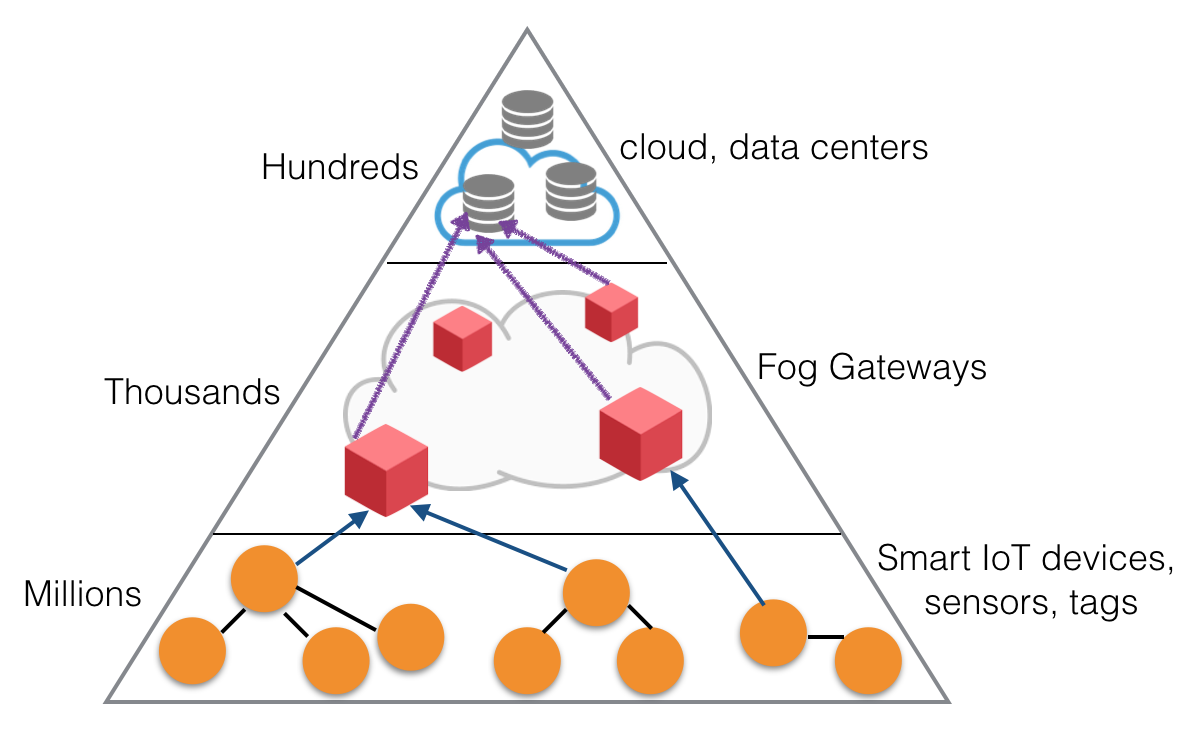
\includegraphics[scale = 0.55]{fog_computing.png}
\caption{The role of the Cloud and Fog play in the delivery of IoT services. \cite{7123563}} 
\label{fig:fog_computing}
\end{figure}

In order to filling the technology gaps in supporting the IoT, a new architecture - Fog - was first introduced. In contrast to traditional cloud model, where many sensors upload raw data directly to a central cloud infrastructure for further processing and analysis, Fog is a highly virtualized platform that provides compute, storage, and networking services between end devices and traditional Cloud Computing data centres, which, typically but not exclusively located at the edge of network \cite{Bonomi:2012:FCR:2342509.2342513}.  Fog consists of heterogeneous, potentially wide-spread and geographically distributed networks of nodes, where a node can be any smart edge device or system that acts as a local control centre for all related sensors and actuators. A Fog in each location can be as small as a single node or as large as required to meet customer demands and a large number of small Fog nodes may form a large Fog system \cite{7498684}. Various services and computing tasks can run on a fog node, depending on how much resource a node owns and application requirements. Applications could let local Fog carry out resource-intensive tasks (M2M interaction, data collection and processing, actuator control, etc.) on behalf of resource-constrained devices when such tasks can not be moved to Cloud due to latency constraints or any other reason, on the other hand let the preprocessed data be consumed by higher tiers, which can be other Fog or the global Cloud for long-term analysis and storage. Due to the characteristics of Fog, it enables IoT applications which require low-latency, location-awareness, real-time interactions and analytics and mobility support. Fog also enhances scalability and resilience of IoT applications by its nature. Figure \ref{fig:fog_computing} illustrates the roles that the Cloud data centres and the Fog play to deliver IoT services to end-users. 

In summary, Fog Computing has the potential to increase the overall performance of IoT applications as it tries to perform part of high level services which are offered by cloud inside the local resources \cite{7123563}. Typical Fog applications include Connected Vehicle (CV), Smart Grid and wireless sensors (actuators) networks \cite{Bonomi:2012:FCR:2342509.2342513}. A real world success of Fog has been discussed in \cite{7498684}, where Barcelona utilized Fog as a uniform platform for all services in their smart city management applications and reduced overall system costs.

Fog Computing provides a new application scenario for this research. Scalability and reliability is still required on a Fog node especially when complex tasks and services being deployed. The Fog node is highly possible a less-constrained embedded device such as the Raspberry Pi \cite{raspberry_pi}, which has more resources than common sensors and actuators yet is much less powerful than the Cloud. Moreover,  since CoAP is a standard M2M protocol, it surely has its use space under a Fog environment. Thus the combination is not only a valid use case in terms of Fog Computing, but also falls into the scope of this research. A detailed evaluation of the proposed CoAP server on Raspberry Pi is stated in chapter \ref{ch5}.

\section{IoT protocols} \label{IoT_protocols}

Many IoT standards have been proposed to facilitate and simplify application programmers' and service providers' jobs. In terms of IoT protocols, various organizations around the world have been created and actively do research in this area. IoT protocols can be classified into different categories, working at different layer, and one category that is cared much in this research is application protocols. In general, current IoT application protocols can be divided into 3 categories: message-oriented, data-oriented, and resource-oriented \cite{7396558}. Representative protocols of the 3 categories are Message Queue Telemetry Transport (MQTT) \cite{mqtt_protocol}, Data Distribution Service for Real Time Systems (DDS) \cite{dds} and The Constrained Application Protocol (CoAP) \cite{coap_protocol}. In this section, these protocols are discussed and compared based on their different architectures, among which, MQTT and DDS are introduced briefly while CoAP is discussed with more details. Reason of choosing CoAP as the protocol used in this research is also stated. 

\subsection{Message-oriented:  Message Queue Telemetry Transport (MQTT)}
Publish/subscribe messaging is one of the most common message-oriented architectures, where subscribers specify their interest in messages of certain type or topic, and receive messages asynchronously once a publisher publishes a message on the registered interest \cite{6918928}. Usually the only property a publisher needs in order to communicate with a subscriber is the name and definition of the data. The publisher does not need any information about the subscribers, and vice versa \cite{pardo2005introduction}. Under message-oriented paradigm, MQTT is outstanding for its simplicity and efficiency, which costs only a small footprint and low power consumption on embedded devices, meanwhile guarantees the reliability and flexibility for message distribution.

MQTT is a messaging protocol that was introduced by Andy Stanford-Clark of IBM and Arlen Nipper of Arcom (now Eurotech) in 1999 and was standardized in 2013 at OASIS \cite{mqtt_protocol}. It aims at connecting embedded devices and networks with applications and middleware. The connection operation uses a routing mechanism (one-to-one, one-to-many, many-to-many) and enables MQTT as an optimal connection protocol for the IoT and M2M \cite{7123563}. 

\begin{figure}[!htbp]
\centering
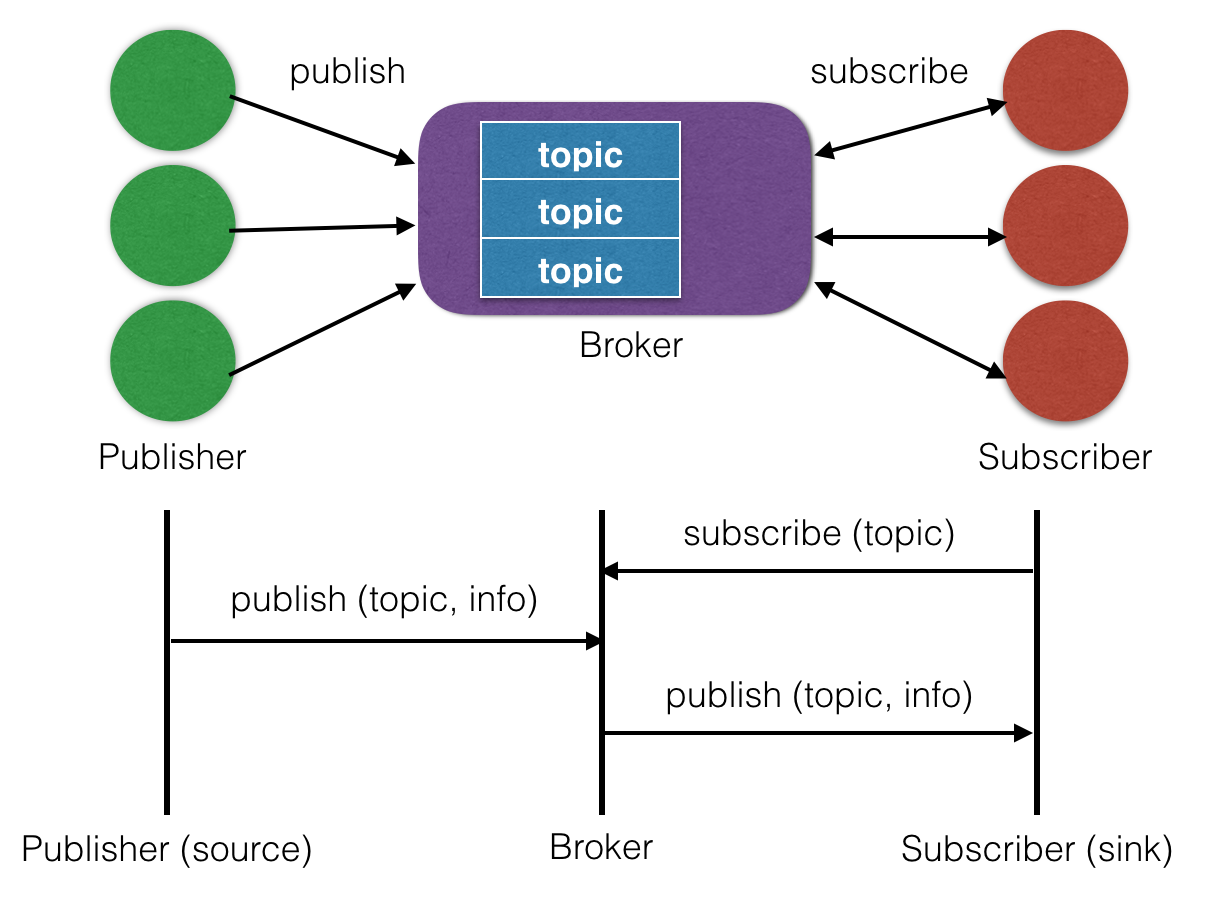
\includegraphics[scale = 0.55]{mqtt.png}
\caption{The architecture of MQTT and its publish/subscribe process}
\label{fig:mqtt}
\end{figure}

MQTT is based on topic based publish-subscribe architecture with a message-broker to bridge between the publishers and subscribers, as shown in figure \ref{fig:mqtt}. An interested device would register as a subscriber for specific topics in order for it to be informed by the broker when publishers publish topics of interest. The publisher acts as a generator of interesting data. After that, the publisher transmits the information to the interested entities (subscribers) through the broker. Furthermore, the broker achieves security by checking authorization of the publishers and the subscribers \cite{4554519}\cite{6504105}.

MQTT exploits the decoupling in space, time and flow as the core of its working philosophy. It supports 3 QoS (quality of service) levels for message delivery with enhanced reliability and has a low header overhead \cite{mqtt_protocol}. MQTT is a connection oriented protocol as the publisher or the subscriber both needs persistent connection to the message broker. It relies on the underlying TCP layer for connection features \cite{6504105}. This in turn can lead to challenges with respect to communication costs. Consequently a UDP based MQTT for sensors (MQTT-S) \cite{4554519} was developed.

\subsection{Data-oriented: Data Distribution Service (DDS)}

Tijero \cite{tijero2012schedulability} and Pardo-Castellote \cite{pardo2005introduction} pointed out that Data Distribution Service for Real Time Systems (DDS) applies a data-oriented/data-centric paradigm. Data-centric communication provides the ability to specify various parameters like the rate of publication, rate of subscription, how long the data is valid, and many others. These Quality of Service (QoS) parameters allow system designers to construct a distributed application based on the requirements for, and availability of, each specific piece of data.

DDS is a publish-subscribe protocol for real-time M2M communications that has been developed by Object Management Group (OMG) \cite{dds}. In contrast to other publish-subscribe application protocols like MQTT, DDS relies on a broker-less architecture and uses multicasting to bring excellent Quality of Service (QoS) and high reliability to its applications \cite{7123563}. Its broker-less architecture fits well with the real-time requirements for IoT and M2M communications. DDS supports 23 QoS policies by which a variety of communication criteria like security, urgency, priority, durability, reliability, etc. can be addressed by the developer \cite{7123563}. In short, DDS has the following advantages \cite{pardo2005introduction}:

\begin{itemize}
\item Based on a simple ``publish-subscribe'' communication paradigm
\item Flexible and adaptable architecture that supports ``auto-discovery'' of new or stale endpoint applications
\item Low overhead -- can be used with high-performance systems
\item Deterministic data delivery
\item Dynamically scalable
\item Efficient use of transport bandwidth
\item Supports one-to-one, one-to-many, many-to-one, and many-to-many communications
\item Large number of configuration parameters that give developers complete control of each message in the system
\end{itemize}

It is important to note that OMG's DDS specification is silent on the wire-protocol. This in turn has led to the problem that DDS products from different vendors face interoperability issues. To overcome these interoperability issues OMG promotes the use of Real-Time Publish-Subscribe protocol (RTPS) \cite{rtps} as a wire-protocol for DDS. RTPS itself relies on the use of UDP and multicast to deliver the data from publishers to subscribers. Depending on the network-topology and routers used, RTPS can deliver impressive throughput. 

An experimental evaluation of two implementations of DDS \cite{4536566} points out that this protocol scales well when the number of nodes is increased. While DDS inspired/compatible protocols have been proposed for wireless and sensor scenarios, there seems to be a lack of successful deployments \cite{7396558}, partly due to its complexity. 


\section{The Constrained Application Protocol} \label{CoAP_intro}

\section{CoAP Implementations} \label{CoAP_imp}